\chapter{O Texto da Tese}

O texto da tese (ou dissertação) é de responsabilidade única do candidato. Claramente o orientador deve orientar a direção desse texto, mas o responsável único, aquele que será aprovado em função do texto é o aluno.

Não é função do orientador corrigir o português dos alunos, ao contrário, como orientador eu espero que os alunos possuam um português de qualidade. Se seu português é ruim, procure um revisor, seja um amigo ou parente voluntário, seja um profissional que você terá que pagar.

Na COPPE o texto pode ser em inglês. Os alunos de doutorado devem realmente escrever sua tese em inglês. Os alunos de mestrado devem tentar.

\section{7 Capítulos }
O número místico 7 aparece aqui para definir o número de capítulos da sua tese, que tem normalmente a seguinte estrutura (meus alunos):
\begin{enumerate}
\item	Introdução: incluindo motivação, introdução ao tema, premissas, questões de pesquisa ou hipótese, objetivos e metas, descrição dos próximos capítulos
\item	Revisão do Problema: incluindo áreas relacionadas, de preferência por meio de Revisão ou Mapeamento Sistemático, em formato top-down, do problema mais geral ao mais específico.
\item	Revisão das Técnicas de Solução ou Metodologia: mostrado, de forma top-down, as teorias, técnicas, tecnologias ou metodologias usadas na solução do problema
\item	Proposta de Solução: na forma teórica ou conceitual
\item	Implementação: descrição da arquitetura e detalhes técnicos
\item	Experimentos: incluindo resultados e comentários
\item	Conclusão: incluindo contribuições gerais (melhoria na solução de um problema) e específicas (bibliotecas de código) e trabalhos futuros.
\end{enumerate}


Isso pode ser reduzido para 5 capítulos:
\begin{enumerate}
    \item	Introdução
   \item	Revisão
   \item	Proposta
   \item	Experimentos
   \item	Conclusão
\end{enumerate}

É curioso que devido a uma superstição iniciada por um professor da PUC que era ligado à numerologia e outras coisas místicas, evitamos teses com 6 capítulos, um número que não é de sorte!

\section{Uma estratégia de escrita}

A tese, ou dissertação, é uma descrição do seu trabalho. Uma boa estratégia para fazer essa descrição é partir das perguntas 5W2H.

Primeiro faça uma lista do que você fez (What).

A partir dessa lista, pergunte para cada coisa que você fez: por que você fez (Why) e como você fez (How).

Isso permitirá gerar um mapa de tudo que deverá aparecer na sua tese.

Quando falo em mapa, digo de forma abstrata, porém não é má ideia construir um mapa conceitual de tudo isso.

As outras perguntas (Where, Who, When, How Much) são menos importantes nesse caso, mas podem dar ideias de trabalho. Por exemplo, onde você fez alguma mudança no código? Quem foi o idealizador de algum algoritmo que você uso? Quanto poder computacional você precisou usar?

Você também pode pensar em 2 Whats: qual o seu problema, qual o seu trabalho. E depois fazer um raciocínio similar. A Figura a seguir mostra uma esquema de raciocínio.

% TODO: \usepackage{graphicx} required
\begin{figure}[hbt]
    \centering
    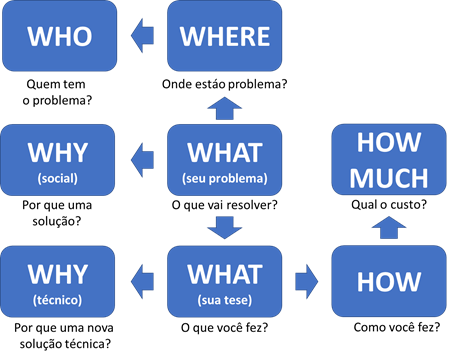
\includegraphics[width=0.7\linewidth]{Images/5w2h}
    \caption{Perguntas que devem ser respondidas antes de iniciar uma tese. Fonte: do autor.}
    \label{fig:5w2h2}
\end{figure}


\section{Quanto as figuras}

As figuras ilustrativas de todos os trabalhos dos alunos devem ser feitas, sempre que isso for possível, em linguagens gráficas da computação. A língua franca da computação atual é UML, que possui uma quantidade muito grande de diagramas que ainda podem ser especializados por meio de estereótipos.

% TODO: \usepackage{graphicx} required
\begin{figure}[hbt]
    \centering
    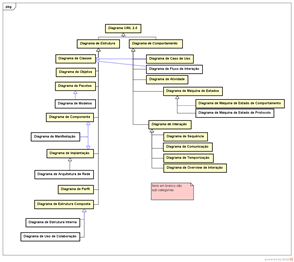
\includegraphics[width=0.7\linewidth]{Images/diagramasuml}
    \caption{Diagramas UML. Fonte: OMG}
    \label{fig:diagramasuml}
\end{figure}


Além dos diagramas de UML, que cobrem quase todos os casos possíveis, outros diagramas também são aceitáveis, como BPMN, Entidades e Relacionamentos e os da família ARIS.

Não use fluxogramas ou caixas genéricas. Fluxogramas não são mais uma linguagem usada em Computação. Diagramas têm que ter significado e é isso que as linguagens padronizadas permitem, ao contrário de caixas genéricas.
